\documentclass[a4paper]{article}

\usepackage[english]{babel}
\usepackage[utf8]{inputenc}
\usepackage{amsmath}
\usepackage{amsfonts}
\usepackage{natbib}
\usepackage{graphicx}
\usepackage[auth-sc,affil-sl]{authblk}
\usepackage[colorinlistoftodos]{todonotes}
\usepackage{hyperref}

\title{User Interface Evaluation of the CP's Website\\ (Proposal)}
\author[1]{Luís  Cruz}
\affil[1]{MAP-i\\ Joint Doctoral Programme in Computer Science}
\date{January 4, 2014}

\begin{document}
\maketitle

\begin{abstract}
  This document proposes an usability test for the website of the company \emph{CP -- Comboios de Portugal}. The company and the website are briefly described, as well as the users focused by the evaluation and the supported tasks. One analytical method and one empirical method are going to be applied in this evaluation: \emph{Heuristic Evaluation} and the \emph{Usability Test}, respectively, both described in this document.
\end{abstract}

\section{Introduction}

This project aims to evaluate the user interface of CP.pt\footnote{Available at: \url{http://www.cp.pt}} --- the official website of \emph{CP - Comboios de Portugal, E.P.E}.

CP is a public portuguese company responsible for rendering national and international passenger rail services. In the year 2012, CP had 4690 employees, transported 122 million passengers and almost 8713 thousand metric tons~\citep{CP2012aa}. They provide 3 main kinds of rail transportation services: \emph{urban} in the cities of Oporto and Lisbon; \emph{National} with regional services and the fast lines of \emph{Alfa Pendular} and \emph{Intercidades}; and \emph{International}.

Through the website, CP's customers can check the timetables, buy tickets, get information about the available lines and special offers and read some news related with CP services. In order to buy tickets, the website provides the \emph{netTicket} service, which requires the customers to have an account in their \emph{myCP} service and it is only available for the long distance trains \emph{Intercidades} and \emph{Alfa Pendular}.

According to the website the graphical interface was optimally designed for windows with $800\times 600$ pixels of resolution. A view of the website is depicted in the figure~\ref{fig:cp_home}, using a window with the same resolution. 

\begin{figure}[h] 
	\centering
	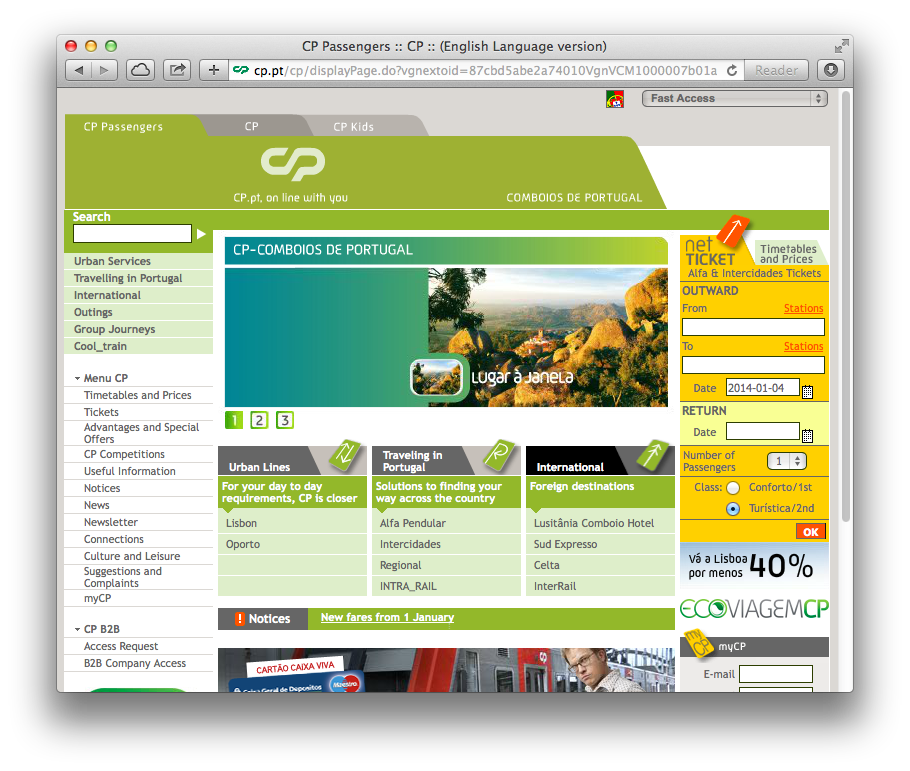
\includegraphics[width=\textwidth]{figures/cp_home}
 	\caption{View of the main page of CP.pt website in a window with resolution $800\times 600$ pixels, using the internet browser Safari Version 7.0.1.}\label{fig:cp_home}
\end{figure}

\section{Users and Context}
\label{sec:users_context}

CP customers vary according to the service provided. Many college students, workers and pensioners use the regional and urban services for small and medium distances. Long distance services are more used by college students that are away from home, tourists, and executive workers. Unfortunately, no official document stating the segmentation of the CP.pt website's users was found.

It is noticeable that CP services have a lot more passengers during school time, which means that students are an important segment of CP's customers. Besides, most of the students have good experience with the WEB, so the CP.pt website is expected to be a great tool to them. Therefore, this usability evaluation will focus in the segment of college students, which might be portuguese citizens as well as foreigners that study or want to study in Portugal and are able to speak English.

Many scenarios can apply for the use of the website by students. Some times they leave the classes earlier and need a way of quickly check if there are other alternative trains that can take them home earlier. Also sometimes there is no direct train to their destination, so they have to catch another in the the middle of the travelling. Another scenario is when the weekend is over and the student has to buy its ticket from home to its university city. Buying it from the website is more convenient since the student can avoid wasting time in the ticket lines and can grant a seat for his trip. Therefore, the following two contexts are considered the most important in terms of usability:

\begin{itemize}
  \item Check the timetable to find any suitable train for the trip and the respective prices.
  \item Buy a ticket for long distance trains with reserved seats.
\end{itemize}

\section{Usability Evaluation}

The evaluation will be taken using two paradigms: \emph{Analytical} and \emph{Empirical}.

\emph{Analytical} methods do not need to involve users --- it is based on inspection methods. Some well known analytical methods are the \emph{Heuristic Evaluation} (HE) proposed by \citet{nielsen1990heuristic}, the \emph{Cognitive Walkthrough} \citep{wharton1994cognitive} and its variant \emph{Streamlined Cognitive Walkthrough} \citep{spencer2000streamlined}.

\emph{Empirical} methods involve the user in the evaluation process through Usability tests, involving \emph{observation} and \emph{query} techniques, and through \emph{controlled experiments} in a more scientific approach. 

In this evaluation, the used analytical method will be the  \emph{Heuristical Evaluation} and the Empirical method will be the \emph{Usability Test}. These methods are described in the next sections.

\subsection{Heuristic Evaluation}

The elected analytical method for this evaluation was the \emph{Heuristic Evaluation}, because it is cheap, intuitive and easy to motivate people to do it~\citep{nielsen1990heuristic}.

This method proceeds by having a small set of evaluators judging the system according to some general principles of interaction design, \emph{heuristics}. It has been shown that a number of evaluators between 3 and 5 provides good results and that there is no point in having more than 10 evaluators \citep{nielsen1990heuristic}. \citet{nielsen1995ten} proposed the 10 most important usability heuristics for User Interface Design:

\begin{itemize}
	\item Visibility of system status

	\item Match between system and the real world

	\item User control and freedom

	\item Consistency and standards

	\item Error prevention

	\item Recognition rather than recall

	\item Flexibility and efficiency of use

	\item Aesthetic and minimalist design

	\item Help users recognize, diagnose, and recover from errors

	\item Help and documentation.
\end{itemize}

Heuristic evaluation was originally developed for evaluators who had some knowledge in usability but who were not necessarily usability experts~\citep{nielsen1990heuristic}, however, it has been showed that the method is also very effective for expert evaluators~\citep{nielsen1992finding}.  


\subsection{Usability Test}

\emph{Usability Tests} involve both observation and query.

\subparagraph{Observation} Observation can be \emph{direct}, by taking notes, or \emph{indirect} through audio/video recording. The users can also be asked to explain what they are doing at each step of the task, known by \emph{think-aloud} (TA) tests, and the system can be logging the activity of the users.
  
\subparagraph{Query} Although the usability test should focus on the performance of users in completing the task, it is beneficial to get the opinion of participants. This is useful because it can provide information about the reason of user's behaviours~\citep{mitchell2007step}. It is made by creating a questionnaire which is good when there are many participants, or through interviews, which are more flexible and can generate ideas and detailed insights that could be lost with questionnaires~\citep{lazar2010research}.

Usability tests require special attention to the following aspects:
\begin{itemize}
\item A careful selection of participants --- it is important to have participants with the same experience level, demographics, and areas of interest, and that will eventually be the end users of the product --- the Screener method is very useful in this phase~\citep{mitchell2007step};
\item Creating a set of tasks that will be given to the participants;
\item Prepare a workplace taking in account any relevant features that might affect the results;
\item Define the experimental design with a procedure, instructions, independent and dependent variables and usability measures to be used.
\end{itemize}

\subparagraph{Common Industry Format} The reports of the usability test will comply the Common Industry Format (CIF) supporting a summative usability evaluation \citep{iusr2006cif}.

When designing a Usability Test it is always a good practice to make a \emph{Pilot Test}. The common strategy is to make an initial walkthrough of the usability test in order to find potential problems of the usability test and make appropriate adjustments~\citep{lewis2006usability}.

%----------------------------------------------------------------------------------------
%	BIBLIOGRAPHY
%----------------------------------------------------------------------------------------

\bibliographystyle{apalike}
\bibliography{bibliography}

%----------------------------------------------------------------------------------------

\end{document}